% !TEX root = ../MasterThesis.tex
\normallinespacing

\chapter{Preliminaries}
\label{sec:preliminaries}

This chapter defines the objects of this
thesis. We fix the class of stochastic systems we aim to reason over, then
introduce certificates and the specifications they witness, along with defining the scope of this thesis. We then present the machine-learning backbone for synthesising certificates and identify its two distinct goals, refutation and verification. Finally, we state the central hypothesis of the thesis.

\section{Notation}
\label{sec:notation}

This section collects the symbols used throughout the thesis; each is defined in
full where it first appears. Calligraphic letters denote sets and spaces
($\aX$, $\aW$, $\aD$, $\mathcal{B}$); blackboard letters denote number sets,
probability, and expectation ($\RN$, $\prob$, $\expe$); fraktur letters are
reserved for the two central structured objects, the Markov chain $\mc$ and the
drift $\drift$; italic letters denote scalars, states, and functions. A
subscript $\theta$ marks a learned object with neural-network parameters
$\theta$, and norms $\|\cdot\|$ are Euclidean unless stated otherwise.

\begin{center}
\mediumlinespacing
\begin{tabular}{lp{9.6cm}}
\hline
\multicolumn{2}{l}{\emph{Stochastic systems}}\\
\hline
$x_t \in \aX \subseteq \RN^d$ & state at time $t$; the state space; $d$ the state dimension \\
$\aX_0,\ \aX_G$ & the initial set; the goal (equilibrium) set \\
$w_t \in \aW,\ \prob_w,\ d_w$ & noise disturbance; the noise space; its distribution; the noise dimension \\
$f : \aX \times \aW \to \aX$ & transition function, with Lipschitz constant $L_f$ \\
$x' \sim P(\,\cdot \mid x)$ & the random successor of $x$; the transition kernel \\
$\indi{E}$ & the indicator of the event $E$ \\
$\mc$ & the induced Markov chain \\
$\Omega,\ \aF_t$ & the sample space of noise sequences $\aW^{\NN}$; the natural filtration $\sigma(x_0, \dots, x_t)$ \\
$\varphi,\ \mc \models \varphi$ & a specification; its satisfaction ($\varphi_{\mathrm{reach}}$ reachability, $\varphi_{\mathrm{term}}$ termination) \\
$\tau$ & the stopping time $\inf\{t \geq 0 : x_t \in \aX_G\}$ \\
$\delta$ & confidence: probabilistic guarantees hold with probability at least $1-\delta$ \\
\hline
\multicolumn{2}{l}{\emph{Certificates and synthesis}}\\
\hline
$\cert,\ \cert_\theta$ & a certificate; a neural certificate with parameters $\theta$ \\
$\varepsilon$ & the decrease margin of the ranking-supermartingale condition \\
$\drift(x)$ & the (stochastic) drift $\expe[\cert(x')] - \cert(x) + \varepsilon$; a certificate is valid iff $\drift \leq 0$ outside $\aX_G$ \\
$D(x)$ & the deterministic drift $\cert(f(x)) - \cert(x) + \varepsilon$ (Chapter~\ref{sec:lipschitz}) \\
$L_\cert,\ L_\drift,\ L_D$ & Lipschitz constants of the certificate and of the two drifts \\
$\aD$ & the learner's training dataset \\
$[z]_+$ & the positive part $\max(0, z)$ \\
$x^\star$ & the worst-case state $\argmax_{x} \drift(x)$ sought in refutation \\
\hline
\multicolumn{2}{l}{\emph{Verification}}\\
\hline
$\mathcal{B},\ B,\ \mathrm{Diam}(B)$ & a grid over $\aX$; one of its cells; the cell's diameter \\
$N$ & the number of grid cells required to certify \\
$b$ & bins per noise dimension in the MILP noise discretisation (the model carries $b^{d_w}$ cells) \\
$m$ & Monte-Carlo successor samples per drift estimate \\
\hline
\end{tabular}
\normallinespacing
\end{center}

Note that three D's coexist by design and are distinguished typographically:
the fraktur $\drift$ is the stochastic drift at the heart of the thesis, the
italic $D$ its deterministic counterpart used in the illustrations of
Chapter~\ref{sec:lipschitz}, and the calligraphic $\aD$ the learner's dataset.
Symbols local to a single method keep the notation of their source and are
introduced in place. These cover algorithm hyperparameters (the whale
optimiser's $a$, $b$, $p$, AdaLipO's online estimate $\hat{k}$, and the
multi-armed bandit's top-$k$), network layer weights $W_\ell$, and
system-specific constants such as the Lyapunov matrix $P$ of the quadratic
certificate $x^\top P x$. This matrix $P$ is distinguished from the transition
kernel by the kernel's explicit conditioning $P(\,\cdot \mid x)$.

\section{Stochastic Systems}

Stochastic systems extend classical dynamical systems to model time-evolving processes subject to
random perturbation. Real-world systems are rarely fully deterministic: sensor noise, actuator
uncertainty, unmodelled dynamics, and environmental disturbances all introduce randomness into
observed trajectories. Two broad modelling philosophies exist. In \textit{robust control},
uncertainty is unknown but bounded, and one designs for the worst-case disturbance within some
admissible set. In \textit{stochastic control}, uncertainty is drawn from a probability
distribution, and one reasons about average-case or probabilistic behaviour. This thesis adopts
the stochastic view, which naturally supports quantitative guarantees of the form ``the system
satisfies property $\varphi$ with probability at least $1 - \delta$.''

Stochastic systems arise across a wide range of application domains. In robotics and
control they model mobile robots navigating under noisy odometry, predictive controllers planning
under Gaussian process uncertainty, and safety-critical systems such as spacecraft rendezvous or
UAV flight envelope protection, where collision avoidance under uncertainty must be formally
guaranteed~\cite{mesbah2016stochastic}. In finance, discrete-time stochastic processes model asset price dynamics, and
probabilistic constraints such as Value-at-Risk underpin portfolio risk management~\cite{jorion2007value}. Stochastic
models also appear in biology (gene regulatory networks, epidemic models)~\cite{allen2008introduction} and cyber-physical
systems (network-induced packet loss)~\cite{schenato2007foundations}. A common thread across these domains is the need not just
to simulate behaviour, but to certify it. That is, to provide formal guarantees that a system
satisfies a safety or performance specification with quantifiable confidence~\cite{lechner2022stability, badings2025logRASM}. The development of
such certificates for stochastic systems is the central concern of this thesis.


\subsection{Discrete-Time Stochastic Dynamical Systems}

The systems of interest are discrete-time stochastic systems, defined as follows:
%
\begin{equation}
    x_{t+1} = f(x_t,\, w_t), \qquad x_0 \in \aX_0,
    \label{eq:stochastic-system}
\end{equation}
%
where $x_t \in \aX \subseteq \RN^d$ is the state at time $t$,
$f : \aX \times \aW \to \aX$ is a (possibly nonlinear) transition function,
$w_t \in \aW$ is a random disturbance drawn i.i.d.\ from a distribution $\prob_w$,
and $\aX_0 \subseteq \aX$ is the set of admissible initial conditions.
A \textit{trajectory} is a realisation $\{x_0, x_1, x_2, \ldots\} \in \aX^\infty$ of this
process. Since $w_t$ is random, a trajectory is itself a random object. One may be interested in behaviour over a finite horizon or asymptotically as $t \to \infty$; the former is more natural for reachability and safety problems
of bounded duration, while the latter arises in stability analysis.

When $\aX$ is equipped with a norm, one can further speak of regularity
properties of the dynamics --- notably the Lipschitz continuity that the
sample-based methods of Section~\ref{sec:sampling-methods} rely on. In particular we assume we have access to the Lipschitz constant of the dynamics $L_f$ (see Chapter~\ref{sec:lipschitz} for more details).

\subsection{Transition Kernels and the Markov Chain}
\label{subsec:kernels}

The dynamics \eqref{eq:stochastic-system} and the noise distribution $\prob_w$
together induce a \emph{transition kernel} $P(\,\cdot \mid x)$: from a state
$x \in \aX$, the probability that the successor $x' := f(x, w)$ with
$w \sim \prob_w$ lands in a measurable set $A \subseteq \aX$ is
%
\begin{equation}
    P(A \mid x) \;:=\; \int_{\aW} \indi{f(x, w) \in A} \; \prob_w(\mathrm{d}w),
    \label{eq:kernel}
\end{equation}
%
the pushforward of the noise distribution through the dynamics. Because the successor depends only on the current state and fresh,
independent noise, the process $\{x_t\}_{t \geq 0}$ is a time-homogeneous
\emph{Markov chain} on $\aX$, which we denote $\mc$ and take as our primary
probabilistic object. Every condition in this thesis is expressed through the
\emph{one-step expectation}
%
\begin{equation}
    \expe_{x' \sim P(\cdot \mid x)}\!\big[\,g(x')\,\big]
    \;=\; \expe_{w \sim \prob_w}\!\big[\,g(f(x, w))\,\big] ,
    \label{eq:onestep}
\end{equation}
%
the expected value of a function $g$ one step into the future from $x$.

For the martingale arguments of Section~\ref{sec:certificates} we occasionally
need to condition on the whole past, not merely the present, and doing so
properly requires fixing the underlying probability space. For a fixed initial
state $x_0$, the trajectory is a deterministic function of the noise sequence,
so we take as sample space the space of noise sequences
$\Omega := \aW^{\NN}$, equipped with the product $\sigma$-algebra $\aF$ and the
product measure $\prob_w^{\otimes\NN}$ of the i.i.d.\ draws. Each state $x_t$
is then a random variable on $\Omega$ through the recursion
\eqref{eq:stochastic-system}, and we write $\prob(\,\cdot \mid x_0)$ and
$\expe[\,\cdot \mid x_0]$ for probability and expectation under this measure.

\begin{definition}[Filtration, adaptedness, stopping time]
\label{def:filtration}
A \emph{filtration} on a probability space $(\Omega, \aF, \prob)$ is an
increasing family $(\aF_t)_{t \geq 0}$ of sub-$\sigma$-algebras
$\aF_0 \subseteq \aF_1 \subseteq \cdots \subseteq \aF$. A process
$(x_t)_{t \geq 0}$ is \emph{adapted} to $(\aF_t)_{t \geq 0}$ if each $x_t$ is
$\aF_t$-measurable, and a random time
$\tau : \Omega \to \NN \cup \{\infty\}$ is a \emph{stopping time} if
$\{\tau \leq t\} \in \aF_t$ for every $t$.
\end{definition}

We equip the chain with its \emph{natural filtration}
$\aF_t := \sigma(x_0, \dots, x_t)$, the smallest $\sigma$-algebra making the
trajectory up to time $t$ measurable --- the information revealed by observing
the process to that point. The chain is adapted by construction, and every
hitting time $\inf\{t \geq 0 : x_t \in A\}$ of a measurable set
$A \subseteq \aX$ is a stopping time, since whether it has occurred by time
$t$ is determined by $x_0, \dots, x_t$ alone; the stopping time $\tau$ of
Section~\ref{subsec:specs} is of exactly this form, which is what entitles us
to apply optional stopping to it. Conditional expectation given $\aF_t$ is
meant in the usual measure-theoretic sense~\cite{williams1991probability}. The
Markov property then makes conditioning on the past coincide with conditioning
on the present: for any measurable, integrable $g$,
%
\begin{equation}
    \expe[\, g(x_{t+1}) \mid \aF_t \,]
    \;=\; \expe[\, g(x_{t+1}) \mid x_t \,]
    \;=\; \expe_{x' \sim P(\cdot \mid x_t)}\!\big[\,g(x')\,\big] .
    \label{eq:markov-property}
\end{equation}
%
Conditioning on the past therefore reduces to the one-step expectation from the
current state, so we work with the compact form \eqref{eq:onestep} throughout and
invoke the filtration only where a martingale theorem explicitly demands it.


\section{Certificates}
\label{sec:certificates}

A \textit{certificate} is a function whose mere existence witnesses that a system
satisfies a property of interest, without ever simulating its trajectories. The
idea originates with Lyapunov~\cite{lyapunov1992general}: to show that a
deterministic system is stable it suffices to exhibit a single scalar function
$\cert : \aX \to \RN$ that decreases along the dynamics, turning an intractable
question about \emph{all} of the infinitely many trajectories into a local,
pointwise condition on one function. This reduction --- from global behaviour to
a checkable inequality --- is the entire appeal of the paradigm, and it is what
makes certificates amenable to automated synthesis and verification.

This section makes the idea precise for stochastic systems. We first fix the
properties we wish to certify (Section~\ref{subsec:specs}); we then develop the
certificate that witnesses them --- the ranking supermartingale --- and reduce
its condition to a single checkable \emph{drift} inequality
(Sections~\ref{subsec:supermartingales}--\ref{subsec:drift}); finally we frame
the verification and synthesis problems this leaves us with
(Section~\ref{subsec:verification}), which the remainder of the thesis is devoted
to solving.

\subsection{Specification Classes}
\label{subsec:specs}

Before one can ask whether a certificate exists, one must fix the property to be
certified. A \emph{specification} $\varphi$ is a property of the trajectories of
the Markov chain $\mc$; we write $\mc \models \varphi$ when the system satisfies
it. Specifications are stated relative to the state space $\aX \subseteq \RN^d$,
an initial set $\aX_0 \subseteq \aX$ from which the system starts, and a
\textit{goal set} (or \textit{equilibrium set}) $\aX_G \subseteq \aX$ that it
should reach; a probabilistic specification additionally carries a confidence
level $\delta$. The two specifications of primary interest in this thesis are the
following.

\paragraph{Reachability.} The \textit{reachability} specification
$\varphi_{\mathrm{reach}}$ holds if, starting from any $x_0 \in \aX_0$, the
trajectory reaches $\aX_G$ with high probability:
%
\begin{equation}
    \prob\!\left(\exists\, t \geq 0 : x_t \in \aX_G \;\middle|\; x_0\right)
    \;\geq\; 1 - \delta
    \qquad \forall\, x_0 \in \aX_0,
    \label{eq:reachability}
\end{equation}
%
for a confidence parameter $\delta \in [0,1)$. When \eqref{eq:reachability} holds
we write $\mc \models \varphi_{\mathrm{reach}}$.

\paragraph{Termination.} The \textit{termination} specification
$\varphi_{\mathrm{term}}$ is stronger: the system reaches $\aX_G$ in
\textit{finite expected time}. Defining the \textit{stopping time}
$\tau := \inf\{t \geq 0 : x_t \in \aX_G\}$, it requires
%
\begin{equation}
    \expe[\tau \mid x_0] \;<\; \infty
    \qquad \forall\, x_0 \in \aX_0.
    \label{eq:termination}
\end{equation}
%
Termination implies reachability with probability one (almost-sure
reachability), but the converse does not hold in general. In practice,
certificates that establish finite expected stopping times are preferable
because they carry quantitative information about \textit{how quickly} the system
reaches its goal, and it is this specification we target throughout.

\paragraph{Beyond reachability.} There exists a wide range of other specifications and certificate types
within the formal methods literature. Of particular note are two recurring specifications defined with respect to an \emph{unsafe set} $\aX_U \subseteq \aX$:
\textit{safety} requires the trajectory to avoid $\aX_U$ (with high probability),
and \textit{reach-avoid} requires it to reach $\aX_G$ while avoiding $\aX_U$ en
route. Both admit certificate characterisations analogous to the supermartingale
conditions developed below~\cite{zikelic2023reachavoid}. The methods we develop extend to safety and
reach-avoid without essential modification.

\subsection{From Lyapunov to Ranking Supermartingales}
\label{subsec:supermartingales}

We now build the certificate that witnesses these specifications, starting from
the deterministic case and relaxing it to the stochastic setting.

\paragraph{Lyapunov functions.} Consider first a \emph{deterministic} system
$x_{t+1} = f(x_t)$ with equilibrium set $\aX_G$. A \textit{Lyapunov function} is
a continuous $\cert : \aX \to \RN_{\geq 0}$ satisfying
%
\begin{align}
    \cert(x) \;&=\; 0 && \forall\, x \in \aX_G, \label{eq:lyap-zero}\\
    \cert(x) \;&>\; 0 && \forall\, x \in \aX \setminus \aX_G, \label{eq:lyap-pos}\\
    \cert(f(x)) \;&<\; \cert(x) && \forall\, x \in \aX \setminus \aX_G. \label{eq:lyap-decrease}
\end{align}
%
The decrease \eqref{eq:lyap-decrease} forces $\cert(x_t)$ to fall along every
trajectory, and since $\cert \geq 0$ vanishes only on $\aX_G$, the system must
reach $\aX_G$. The certificate has reduced a global question --- does every
trajectory converge? --- to a local, pointwise inequality.

\paragraph{Supermartingales.} Under noise the successor is random, so demanding a
pointwise decrease at every realisation is too strong: a single noisy step may
raise $\cert$. The natural relaxation asks $\cert$ to decrease \emph{in
expectation}. Writing $x'$ for the random successor of $x$, the function $\cert$
is a \emph{supermartingale} for $\mc$ if
%
\begin{equation}
    \expe_{x' \sim P(\cdot \mid x)}[\cert(x')] \;\leq\; \cert(x)
    \qquad \forall\, x \in \aX \setminus \aX_G .
    \label{eq:supermartingale-condition}
\end{equation}
%
By the Markov property \eqref{eq:markov-property} this is precisely the classical
martingale condition $\expe[\cert(x_{t+1}) \mid \aF_t] \leq \cert(x_t)$, so
$\{\cert(x_t)\}$ is a supermartingale in the usual sense and its convergence
theory applies: a non-negative supermartingale that vanishes only on $\aX_G$ has
$\cert(x_t) \to 0$ almost surely, and hence reaches the goal with probability
one, $\mc \models \varphi_{\mathrm{reach}}$~\cite{williams1991probability}.

\paragraph{Ranking supermartingales.} Almost-sure reachability says the system
arrives, but not how quickly. Strengthening the relaxation to a \emph{strict}
expected decrease by a fixed margin $\varepsilon > 0$,
%
\begin{equation}
    \expectation \;\leq\; \cert(x) - \varepsilon
    \qquad \forall\, x \in \aX \setminus \aX_G ,
    \label{eq:ranking-supermartingale}
\end{equation}
%
makes $\cert$ a \emph{ranking supermartingale}. By Doob's optional stopping
theorem~\cite{williams1991probability} it bounds the expected stopping time,
$\expe[\tau \mid x_0] \leq \cert(x_0)/\varepsilon < \infty$, so the system
terminates in finite expected time \eqref{eq:termination},
$\mc \models \varphi_{\mathrm{term}}$, with an explicit bound. \textbf{The ranking supermartingale is the certificate this
thesis is concerned with.} It delivers the quantitative termination guarantee of
Section~\ref{subsec:specs}, and its defining condition collapses to a single inequality a machine can check.

\subsection{The Drift Condition}
\label{subsec:drift}

The ranking condition \eqref{eq:ranking-supermartingale} still mixes the
certificate, the dynamics, and the margin across an inequality. Moving everything
to one side turns it into a single scalar function of the state --- the
\emph{drift} ---
%
\begin{equation}
    \drift(x) \;:=\; \expe_{x' \sim P(\cdot \mid x)}[\cert(x')] - \cert(x) + \varepsilon ,
    \label{eq:drift-def}
\end{equation}
%
the expected one-step change in $\cert$ together with the required margin. The
ranking supermartingale condition \eqref{eq:ranking-supermartingale} is then
\emph{exactly} the statement that this drift is non-positive everywhere outside
the goal:
%
\begin{equation}
    \drift(x) \;\leq\; 0 \qquad \forall\, x \in \aX \setminus \aX_G .
    \label{eq:goal}
\end{equation}
%
Equation~\eqref{eq:goal} is the central object of this thesis. A candidate
$\cert$ is a valid certificate precisely when its expected drift is non-positive
at every state outside the goal set; \textbf{establishing \eqref{eq:goal} for all
$x$ --- not merely at the finitely many states we can sample --- is the single
claim that every verifier and refuter in the sequel is built to settle.}
Table~\ref{tab:certificate-conditions} collects the three conditions and the
guarantees they induce.

\begin{table}[h]
\centering
\small
\begin{tabular}{lll}
\hline
\textbf{Certificate} & \textbf{Condition ($x \in \aX \setminus \aX_G$)} & \textbf{Guarantee} \\
\hline
Lyapunov function & $\cert(f(x)) < \cert(x)$ & convergence to $\aX_G$ (deterministic) \\
Supermartingale & $\expe_{x'\sim P(\cdot\mid x)}[\cert(x')] \leq \cert(x)$ & a.s.\ reachability, $\mc \models \varphi_{\mathrm{reach}}$ \\
Ranking supermart. & $\drift(x) \leq 0$ & finite expected termination, $\mc \models \varphi_{\mathrm{term}}$ \\
\hline
\end{tabular}
\caption{The certificate conditions and the guarantees they induce; throughout
$\cert \geq 0$ with $\cert = 0$ on $\aX_G$. This thesis targets the ranking
supermartingale, whose condition is the drift inequality \eqref{eq:goal}.}
\label{tab:certificate-conditions}
\end{table}

\subsection{Verification Problem Formulations}
\label{subsec:verification}

The certificate conditions above leave us with two distinct computational
problems. Throughout, a \emph{candidate} is a function
$\cert : \aX \to \RN_{\geq 0}$ with $\cert = 0$ on $\aX_G$, and validity means
the drift condition \eqref{eq:goal}.

\begin{definition}[The verification problem]
\label{def:verification}
Given a Markov chain $\mc$ on $\aX$ with goal set $\aX_G$, a margin
$\varepsilon > 0$, and a candidate $\cert$, decide whether
%
\begin{equation*}
    \drift(x) \;\leq\; 0 \qquad \forall\, x \in \aX \setminus \aX_G ,
\end{equation*}
%
returning \textup{\textsc{Verified}} if so, and otherwise a \emph{counterexample}: a
state $x^\star \in \aX \setminus \aX_G$ with $\drift(x^\star) > 0$.
\end{definition}

For a fixed $\cert$ this is a \textit{constraint satisfaction} problem over a
continuous domain; the challenge is that the condition must be discharged at
uncountably many states, not merely those we can sample.

\begin{definition}[The synthesis problem]
\label{def:synthesis}
Given $\mc$, $\aX_G$ and $\varepsilon > 0$, together with a hypothesis class
$\aV \subseteq \{\cert : \aX \to \RN_{\geq 0} \mid \cert = 0 \text{ on } \aX_G\}$,
find a candidate $\cert \in \aV$ satisfying the drift condition
\eqref{eq:goal}.
\end{definition}

Synthesis is strictly harder than verification: any solution must in
particular be verifiable, and the search ranges over the whole class $\aV$
rather than interrogating a single candidate. The choice of $\aV$ is the
central design decision --- this thesis takes $\aV = \{\cert_\theta : \theta
\in \Theta\}$, the class of neural networks over a fixed architecture ---
and the paradigms below differ exactly in that choice.

\paragraph{Approaches to synthesis.} Several paradigms have been developed to
address these problems.

\textit{Sum-of-squares (SOS) programming}~\cite{parrilo2000} restricts $\cert$ to
the class of polynomials and encodes the certificate conditions as polynomial
non-negativity constraints, which can be relaxed to a semidefinite programme
(SDP) via the Positivstellensatz. SOS methods provide formal soundness
guarantees and are well-suited to low-dimensional polynomial systems, but scale
poorly with state dimension and cannot represent non-polynomial dynamics.

\textit{Template-based synthesis} instead fixes a parametric form for $\cert$ ---
for instance a linear or piecewise-linear combination of fixed basis functions
--- and solves for its coefficients, reducing synthesis to a linear or convex
feasibility programme when the template and dynamics are compatible. Templates
are cheap and interpretable, but only as expressive as the chosen basis, and
finding a basis that admits a valid certificate is itself the hard part.

Both paradigms fix the hypothesis class in advance and trade expressiveness for
scalability. The alternative this thesis pursues is to \emph{learn} the
certificate as a neural network, gaining the expressive power to handle
high-dimensional and non-polynomial systems at the cost of the closed-form
soundness guarantee --- a guarantee recovered through the counterexample-guided
loop developed in the next section.


\section{Counterexample-Guided Inductive Synthesis}
\label{sec:cegis}

The neural route replaces the fixed hypothesis class of the previous section
with a \emph{neural certificate} $\cert_\theta$: a neural network with parameters
$\theta$. Its universal approximation capacity makes the class expressive enough
for high-dimensional, non-polynomial, and even learned dynamics, but it forfeits
the closed-form soundness of SOS or template synthesis --- fitting $\cert_\theta$
on a finite set of sampled states says nothing about the uncountably many states
between them. \emph{Counterexample-guided inductive synthesis}
(CEGIS)~\cite{chatterjee2023learnerverifier, abate2021fossil} recovers a sound
guarantee by interleaving learning with formal checking, as illustrated in
Figure~\ref{fig:cegis_certificate}.

\paragraph{The loop.} CEGIS seeks parameters $\theta$ for which $\cert_\theta$
witnesses the specification, i.e.\ for which the drift condition
\eqref{eq:goal} holds: $\drift(x) \le 0$ for all $x \in \aX \setminus \aX_G$. It
alternates two components. A \emph{learner} takes a finite dataset
$\aD \subseteq \aX$ of states and trains $\cert_\theta$ to satisfy the drift
condition \emph{on $\aD$}. A \emph{verifier} then checks whether the trained
$\cert_\theta$ satisfies it on the \emph{entire} continuous domain. If the verifier succeeds, the candidate is a valid certificate
and the loop halts. If it fails, it returns one or more \emph{counterexamples}
--- states at which a condition is violated --- which are appended to $\aD$
before the learner is invoked again. Each counterexample forbids the current
flaw, so the loop makes monotone progress towards soundness.

\paragraph{Learner.} The learner performs empirical risk minimisation over the
current dataset: it fits the parameters $\theta$ so that the candidate satisfies
the drift condition at the sampled states. With $[z]_+ := \max(0, z)$ the
positive part, it minimises the empirical risk
%
\begin{equation}
    \ell(\theta) \;=\; \frac{1}{|\aD|} \sum_{x \in \aD} \big[\, \drift_\theta(x) \,\big]_+ ,
    \label{eq:cegis-loss}
\end{equation}
%
a hinge penalty that vanishes exactly where the drift $\drift_\theta$ of
$\cert_\theta$ (cf.\ \eqref{eq:drift-def}) is non-positive. When the one-step
expectation inside $\drift_\theta$ has no closed form it is estimated by a
Monte-Carlo average over $m$ successor samples $x'_1, \dots, x'_m \sim P(\cdot
\mid x)$. Driving \eqref{eq:cegis-loss} to zero certifies nothing on its own: an
empirical risk over finitely many states is silent about the continuum between
them, which is exactly why a verifier is needed.

\paragraph{Verifier.} The verifier discharges the drift condition \eqref{eq:goal}
 either certifying it, so that $\cert_\theta$ proves $\mc \models \varphi_{\mathrm{term}}$, or
returning a counterexample $x$ with $\drift(x) > 0$. Because the claim quantifies
over a continuous domain, the verifier must reason soundly about the gaps between
sampled states.



\begin{figure}[t]
    \centering
    \resizebox{\columnwidth}{!}{%
    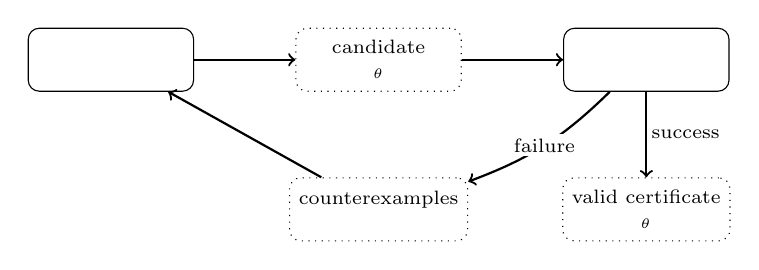
\begin{tikzpicture}[
        box/.style={draw, rounded corners, align=center, minimum width=2.1cm, minimum height=0.8cm, font=\scriptsize},
        outputnode/.style={draw, dotted, rounded corners, align=center, minimum width=2.1cm, minimum height=0.8cm, font=\scriptsize},
        arr/.style={->, thick},
        % white-backed edge label so it never collides with an arrow or a box
        lbl/.style={font=\scriptsize, fill=white, inner sep=1.5pt}
    ]
        % columns at x = 0, 3.4, 6.8 ; rows at y = 0, -1.9 (widen these to add space)
        \node[box] (learner) at (0,0) {$\learner$};
        \node[outputnode] (candidate) at (3.4,0) {candidate\\$\cert_\theta$};
        \node[box] (verifier) at (6.8,0) {$\verifier$};

        \node[outputnode] (cex) at (3.4,-1.9) {counterexamples\\$\aD$};
        \node[outputnode] (valid) at (6.8,-1.9) {valid certificate\\$\cert_\theta$};

        \draw[arr] (learner) -- (candidate);
        \draw[arr] (candidate) -- (verifier);
        \draw[arr] (verifier) -- node[lbl, right] {success} (valid);
        \draw[arr] (verifier) to[bend left=12] node[lbl, pos=0.5] {failure} (cex);
        \draw[arr] (cex) -- (learner);
    \end{tikzpicture}%
    }
    \caption{Learner--verifier loop for neural certificate synthesis.}
    \label{fig:cegis_certificate}
\end{figure}

\paragraph{Two goals within one loop.} The loop of
Figure~\ref{fig:cegis_certificate} asks its verifier to discharge two formally
distinct problems. While the candidate is invalid, the loop needs only to
\emph{refute} it. This is an \emph{existential} search for some counterexample
(Definition~\ref{def:verification}), which may stop at the first witness and need
not be sound, since a spurious near-miss costs only a wasted training point. Once
the candidate is valid, the loop needs to \emph{verify} it. This is a
\emph{universal} claim that no counterexample exists anywhere, which must clear
the whole domain and must be sound, since a single missed violation invalidates
the certificate. The prevailing practice nonetheless discharges both with a
\emph{single} method, running the sound verifier every round.

\medskip
\noindent\textbf{Hypothesis.}\enspace \emph{Because refutation and verification
are distinct computational tasks, giving each its own dedicated algorithm yields a substantial speed-up over discharging
both with one method.} The remainder of this thesis
develops the two tasks separately, verification in
Chapter~\ref{chap:verification} and refutation in Chapter~\ref{chap:refutation},
and Chapter~\ref{chap:streamlining} tests the hypothesis directly, pairing a fast
refuter pre-screen with a sound verifier and measuring the speed-up.


\newpage